\section{OpenFlow}
\subsection{OpenFlow의 개념}
    OpenFlow는 네트워크 장치의 Control Plane과 Data Plane 간의 인터페이스 위한 표준 통신 프로토콜이다. SDN을 실현하기 위한 가장 적합한 기술로 평가되었으며, 현재 SDN 컨트롤러와 네트워크 장치간의 인터페이스 규격으로 사용되고 있다. \\
    \vspace{-4mm}
    \begin{figure}[!h]\centering
		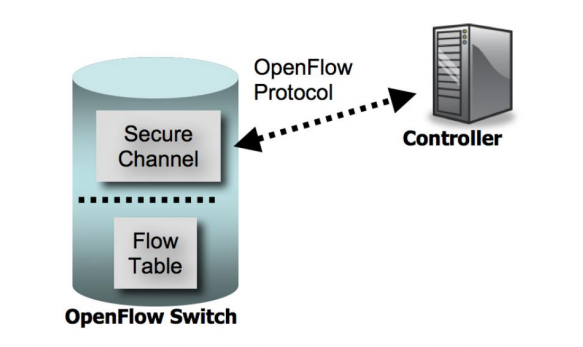
\includegraphics[width=.65\textwidth]{image/week05/2-1.png}
		\caption{\small OpenFlow Structure}
		\vspace{-10pt}
    \end{figure}
    
    OpenFlow의 구성요소는 다음과 같다. \\
    
    \subsubsection*{OpenFlow Controller}
    OpenFlow Protocol을 사용하여 네트워크 장치 설정 및 어플리케이션 최적 경로 설정하는 소프트웨어이다. 상위 응용이나 정책 요구에 따라 차별화된 포워딩 및 패킷 처리 룰을 결정하여 하위의 OpenFlow Switch에 전달한다. \\
    
    \subsubsection*{OpenFlow Protocol}
     OpenFlow Controller와 Switch가 통신하기 위한 개방형 표준 인터페이스 \\
     
    \subsubsection*{OpenFlow Switch}
    OpenFlow Controller에서 받은 Flow Table대로 패킷 포워드와 조작, 통계 수집, 터널 캡슐화/비캡슐화 등의 기능을 수행한다. \\
    
    \subsubsection*{Flow Table}
    OpenFlow Switch가 패킷을 제어하는 정보가 들어있는 테이블이다. Rule, Action, Stats로 구성된다. Rule은 플로우를 정의하는 패킷 헤더 정보를 갖는다. Action은 입력 패킷 정보가 Rule에 정의된 정보와 일치할 때 패킷을 어떻게 처리할지에 대한 정보를 담고 있다. Action에 따라 패킷을 경로에 맞게 전달하거나 전달 경로를 변경하거나, 더 이상 전달되지 않게 차단할 수 있다. Stats은 각 플로우별로 Rule이 일치하는 패킷이 얼마나 많이 입력되었는지를 보여준다. \\
    \vspace{-4mm}
    \begin{figure}[!h]\centering
		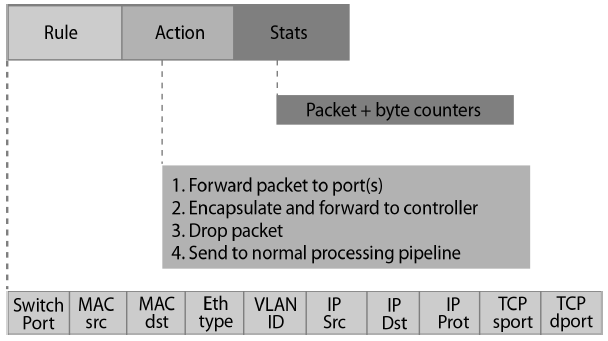
\includegraphics[width=.65\textwidth]{image/week05/2-2.png}
		\caption{\small Flow Table}
		\vspace{-10pt}
    \end{figure}
    
     \subsubsection*{Secure Channel}
     OpenFlow Controller와 Switch간의 통신을 위한 보안 채널 \\
     
\subsection{OpenFlow 기반 SDN의 동작}
    패킷이 발생하면 제일 먼저 OpenFlow Switch의 Flow Table에 해당 패킷에 대한 정보가 있는지 확인한다. 일치하는 정보가 있다면 그에 맞추어 패킷을 처리하고, 정보가 없다면 해당 패킷에 대한 제어 정보를 OpenFlow Controller에 요청한다. \\
    제어 정보 요청을 받은 OpenFlow Controller는 내부의 패킷 제어 정보를 확인하고, 그 결과를 OpenFlow Switch에 전달한다. 이 OpenFlow Controller 내부의 패킷 제어 정보는 외부 프로그램에서 API를 통해 입력할 수 있다. \\
    패킷 제어 정보를 전달 받은 OpenFlow Switch는 전달 받은 정보를 Flow Table에 저장한다. 이후 동일한 패킷이 발생하면 OpenFlow Controller에 요청할 필요 없이 Flow Table 정보에 따라 패킷을 처리한다. \\
\newpage